\documentclass{article}

\usepackage{tikz}
\usepackage{pgfplots}
\usepgfplotslibrary{fillbetween}

\begin{document}
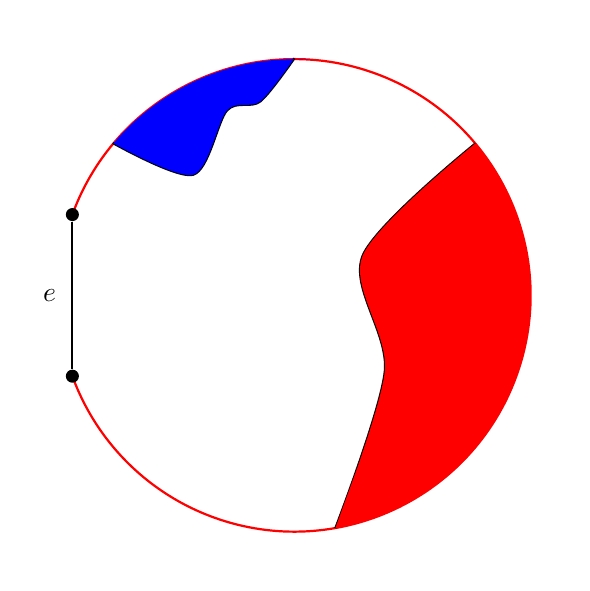
\begin{tikzpicture}[thick,every node/.style={circle,scale=.5,fill}]

\draw[red,name path=arc]  (160:3) arc (160:-160:3);

\node (e1) at (160:3) {};
\node (e2) at (-160:3) {};

\draw(e1) -- node[fill=none,left,scale=2] {$e$} (e2);

\draw[name path=A] plot [smooth] coordinates {(140:3.01) (130:2) (110:2.5) (100:2.5) (90:3.01)};
\draw[name path=B] plot [smooth] coordinates {(40:3.001) (30:1) (-40:1.5) (-80:3.001)};

\tikzfillbetween[of=A and arc,on layer=,split,every even segment/.style={fill=none,draw=none}]{blue,opacity=50}


\tikzfillbetween[of=B and arc,on layer=,split,
	every even segment/.style={fill=none,draw=none},
]{red,opacity=50}
\end{tikzpicture}
\end{document}
